%-------------------------
% Resume in Latex
% Author : Zakaria TOZY
%------------------------

\documentclass[11pt,a4paper]{article}

\usepackage{latexsym}
\usepackage[empty]{fullpage}
\usepackage{titlesec}
\usepackage{marvosym}
\usepackage[usenames,dvipsnames]{color}
\usepackage{verbatim}
\usepackage{enumitem}
\usepackage[hidelinks]{hyperref}
\usepackage{fancyhdr}
\usepackage[english,french]{babel}
\usepackage{tabularx}
\usepackage[utf8]{inputenc}
\usepackage[left=0.5in, right=0.5in, top=0.1in, bottom=0.2in]{geometry}
\usepackage{exscale}  % Pour la commande \HUGE

\usepackage{fontawesome}
\usepackage[scale=0.90,lf]{FiraMono}

\definecolor{light-grey}{gray}{0.83}
\definecolor{dark-grey}{gray}{0.3}
\definecolor{text-grey}{gray}{.08}

\DeclareRobustCommand{\ebseries}{\fontseries{eb}\selectfont}
\DeclareTextFontCommand{\texteb}{\ebseries}

\usepackage{contour}
\usepackage[normalem]{ulem}
\renewcommand{\ULdepth}{1.8pt}
\contourlength{0.8pt}
\newcommand{\myuline}[1]{%
  \uline{\phantom{#1}}%
  \llap{\contour{white}{#1}}%
}

\usepackage{tgheros}
\renewcommand*\familydefault{\sfdefault} 
\usepackage[T1]{fontenc}

\usepackage{graphicx}

\pagestyle{fancy}
\fancyhf{} 
\fancyfoot{}
\renewcommand{\headrulewidth}{0pt}
\renewcommand{\footrulewidth}{0pt}

\urlstyle{same}

\raggedbottom
\raggedright
\setlength{\tabcolsep}{0in}

\titleformat{\section}{
    \bfseries \vspace{-4pt} \raggedright \normalsize
}{}{0em}{}[\color{light-grey} {\titlerule[1pt]} \vspace{-2pt}]

\newcommand{\resumeItem}[1]{
  \item\footnotesize{
    {#1 \vspace{-1pt}}
  }
}

\newcommand{\resumeSubheading}[4]{
  \vspace{2pt}\item
    \begin{tabular*}{\textwidth}[t]{l@{\extracolsep{\fill}}r}
      {\footnotesize\textbf{#1}} & {\footnotesize#2} \\
      {\footnotesize\textit{#3}} & {\footnotesize\textit{#4}} \\
    \end{tabular*}\vspace{2pt}
}

\newcommand{\resumeProjectHeading}[2]{
  \item
  {\footnotesize#1} \hfill {#2}
}

\newcommand{\resumeSubItem}[1]{\resumeItem{#1}\vspace{-4pt}}

\renewcommand\labelitemii{$\vcenter{\hbox{\tiny$\bullet$}}$}

\newcommand{\resumeSubHeadingListStart}{\begin{itemize}[leftmargin=0in, label={}]}
\newcommand{\resumeSubHeadingListEnd}{\end{itemize}}
\newcommand{\resumeItemListStart}{\begin{itemize}[label={\textbullet}]}
\newcommand{\resumeItemListEnd}{\end{itemize}\vspace{0pt}}

\color{text-grey}

\begin{document}

\begin{flushleft}
  \begin{minipage}[c]{0.2\textwidth}
    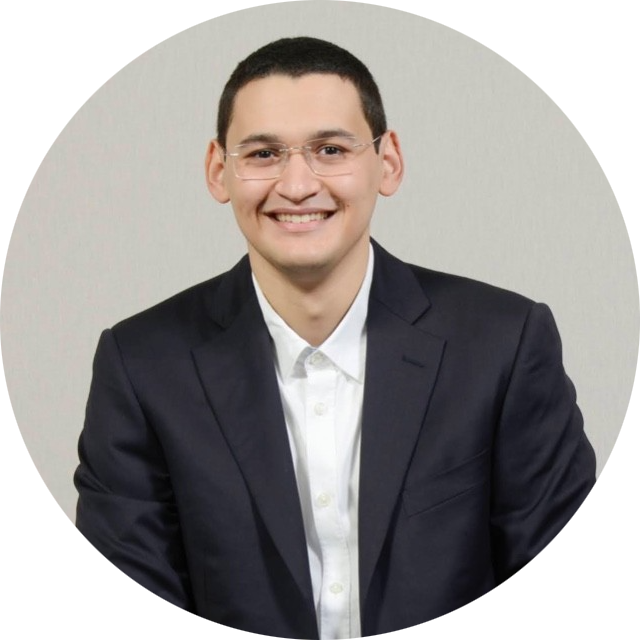
\includegraphics[width=3cm]{images/profilpicture.png}
  \end{minipage}%
  \begin{minipage}[c]{0.8\textwidth}
    {\Huge \textbf{Zakaria TOZY}} \\[5pt]
    {\Large \textbf{Data Engineer | CDI}}
  \end{minipage}
\end{flushleft}

\vspace{-5pt}

\begin{center}
    \small \faPhone\ \texttt{0617407077} \hspace{1pt} $|$
    \hspace{1pt} \faEnvelope\ \texttt{zakaria.tozy@icloud.com} \hspace{1pt} $|$
    \hspace{1pt} \faLinkedin\ \texttt{zakaria-tozy} \hspace{1pt} $|$
    \hspace{1pt} \faMapMarker\ \texttt{Paris} \hspace{1pt} $|$
    \hspace{1pt} \faGithub\ \texttt{github.com/zack242} \\ \vspace{0pt}
\end{center}

\begin{itemize}[leftmargin=0in, label={}]
\footnotesize{\item{
Computer Science and Data Science Engineer with a dual degree (ECE Paris/Polytechnique), combining technical expertise in data engineering with experience in financial data processing at AXA IM. Seeking to contribute to innovative projects.
}}
\end{itemize}

\section{SKILLS}
\begin{itemize}[leftmargin=0in, label={}]
\footnotesize{\item{
{\footnotesize\textbf{Programming}:} {\footnotesize Python, SQL, Java, JavaScript, C++, C{\#}} \\
\vspace{3pt}
{\footnotesize\textbf{Data Cloud Engineering}:} {\footnotesize PySpark, ETL, Data Pipelines, Databricks, Snowflake, GCP, Azure, S3, dbt, Airflow} \\
\vspace{3pt}
{\footnotesize\textbf{Machine Learning}:} {\footnotesize Scikit-Learn, NLP, Computer Vision, Deep Learning, LLM, API Integration} \\
\vspace{3pt}
{\footnotesize\textbf{Devops}:} {\footnotesize Docker, CI/CD, Git, Scrum} \\
\vspace{3pt}
{\footnotesize\textbf{Soft Skills}:} {\footnotesize Problem Solving, Team Collaboration, Technical Leadership, Innovation Mindset} \\
\vspace{3pt}
{\footnotesize\textbf{Languages}:} {\footnotesize French (Native), Arabic (Native), English (Fluent - TOEIC 875)}
}
}
\end{itemize}

\section{EDUCATION}
\resumeSubHeadingListStart
    \resumeSubheading
      {École Centrale d'Électronique (ECE Paris)}
      {January 2024}
      {Engineering Degree in Computer Science and Big Data Analytics}
      {Top 5\% of class}
      \resumeItemListStart
        \resumeItem{Specialization: Programming, Databases, Electronics, DevOps}
      \resumeItemListEnd
    \resumeSubheading
      {Institut Polytechnique de Paris (École Polytechnique)}
      {January 2024}
      {Master's Degree in Data Science}
      {With Highest Honors}
      \resumeItemListStart
        \resumeItem{Specialization: Machine Learning, Big Data, Cloud Infrastructure, Deep Learning, NLP}
      \resumeItemListEnd
  \resumeSubHeadingListEnd

\section{EXPERIENCE}
\resumeSubHeadingListStart
    \resumeSubheading
      {AXA Investment Managers - AXA IM}{August 2023 --- January 2024}
      {Data Engineer/Data Analyst Intern}{Paris}
      \resumeItemListStart
        \resumeItem{Designed and implemented data pipelines for business and historical data ingestion and management}
        \resumeItem{Optimized data model and migrated distribution pipelines for financial reporting of €844 billion in assets}
        \resumeItem{Tested new Databricks clusters and created a PoC for sensitive data anonymization}
        \resumeItem{Built dashboards and calculated KPIs for distributed vision (ME, OV, CIS, FX)}
      \resumeItemListEnd
    \resumeSubheading
      {Kalima Blockchain and IoT}{April 2022 --- August 2022}
      {Software Engineer Intern}{Paris}
      \resumeItemListStart
        \resumeItem{Developed a proprietary Kalima blockchain explorer in Java/LevelDB (+1000 transactions per second)}
        \resumeItem{Implemented new administration features for Kalima proprietary blockchain using Node.js}
        \resumeItem{Designed and developed a multi-signature authentication system for DApps (Decentralized Applications) on Kalima blockchain}
      \resumeItemListEnd
    \resumeSubheading
      {Le Crédit Lyonnais - LCL}{January 2020 --- February 2020}
      {IT Intern}{Paris}
      \resumeItemListStart
        \resumeItem{Studied Microsoft Office migration from 2010 to 2016 and analyzed its impact on business processes}
        \resumeItem{Developed and executed test procedures on 23,000 workstations}
      \resumeItemListEnd
  \resumeSubHeadingListEnd

\section{PROJECTS}
\resumeSubHeadingListStart
    \resumeProjectHeading
      {\textbf{Bitcoin Analysis}} {}
      \resumeItemListStart
        \resumeItem{Created a data pipeline using Python, SQL, Airflow, dbt, and Snowflake for Bitcoin transaction analysis, processing over 1 million transactions per day}
      \resumeItemListEnd
    \resumeProjectHeading
      {\textbf{Twitter Real-time Analysis}} {}
      \resumeItemListStart
        \resumeItem{Developed a real-time visualization system for Twitter streams by subjects using Kafka and KNN (K-Nearest Neighbors) algorithm}
      \resumeItemListEnd
    \resumeProjectHeading
      {\textbf{Energy Disaggregation with Capgemini}} {}
      \resumeItemListStart
        \resumeItem{Extracted the temperature-sensitive component of energy consumption to forecast future demand in France}
      \resumeItemListEnd
\resumeSubHeadingListEnd


\end{document} 